% two-flop synchroniser
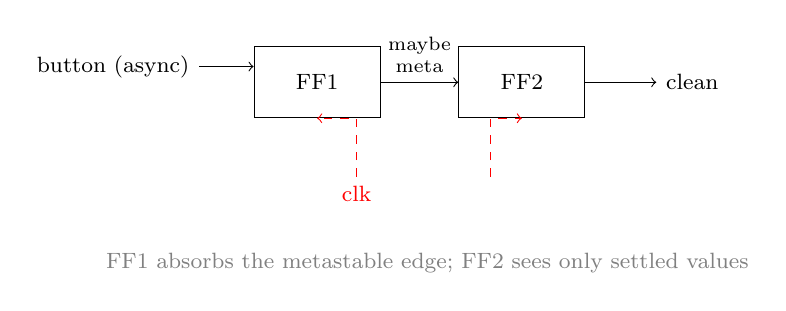
\begin{tikzpicture}[font=\footnotesize, cell/.style={draw, minimum width=1.6cm, minimum height=0.9cm}]
\node[cell] (f1) at (0,0) {FF1};
\node[cell] (f2) at (2.6,0) {FF2};
\draw[->] (-1.5,0.2) node[left] {button (async)} -- (f1.west |- 0,0.2);
\draw[->] (f1.east) -- node[above, font=\scriptsize, align=center] {maybe\\meta} (f2.west);
\draw[->] (f2.east) -- ++(0.9,0) node[right] {clean};
\draw[->, dashed, red] (0.5,-1.2) node[below] {clk} |- (f1.south);
\draw[->, dashed, red] (2.2,-1.2) |- (f2.south);
\node[gray] at (1.4,-2.3) {FF1 absorbs the metastable edge; FF2 sees only settled values};
\end{tikzpicture}
